\section{Introduction}

Retail banking is moving from a product-centred model to a relationship-centred model. A customer can keep an account open while moving daily payments, salary inflows, savings, or credit usage elsewhere. That distinction matters: account ownership is not proof of active use or loyalty. The World Bank's 2025 Global Findex covers roughly 148,000 adults in 141 economies and measures how adults use accounts to pay, save, borrow, and manage shocks \citep{worldbank2025findex}. The business question is therefore not simply ``who has an account?'' It is ``whose relationship is weakening, what service problem may be visible, and what should the bank test before the customer leaves?''

The problem is timely because customers can compare digital experiences quickly. A 2025 retail-banking survey reported that more than one third of customers had switched banks in the previous five years, with better digital experience a more common priority than rate competition \citep{baringa2025}. Acquisition is also expensive: Curinos estimated that the cost to acquire a checking customer reached US\$559 in 2025 \citep{curinos2025}. These industry figures motivate retention work; they are not financial estimates for the bank represented by this dataset.

This project builds a reproducible customer-intelligence prototype for a digital bank. It combines a static Kaggle churn dataset with a Python-generated, six-month behavioural extension. The product has four aims: describe customers and their relationship with the bank; segment behaviour without using churn as an input; estimate historical churn propensity only after appropriate validation; and convert evidence into consent-aware retention experiments. The dataset has no real event history or temporal churn window. Hence, the project does not claim to predict next-quarter churn or to measure realised campaign uplift.

\section{Banking background and decision context}

\subsection{What churn means in this project}

The source label records historical relationship exit. It cannot distinguish account closure, product attrition, temporary dormancy, balance flight, or preventable churn. A customer may own several products, remain funded while inactive, or close one card while retaining a deposit relationship. The report therefore treats churn as a static historical label and uses it only for descriptive cross-tabs until a valid classification protocol is complete.

\subsection{The operating decision}

The retention team needs an action queue, not a decorative score. A safe decision flow is: confirm consent and contact cap; suppress customers with unresolved service cases; place eligible customers into a behavioural segment; assign a treatment/control arm; measure activity, complaints, opt-outs and retention; then stop, iterate or scale. Customer service takes precedence over promotion when a case is open. Gender and country are used only for aggregate fairness checks.

\section{Data overview, provenance and analysis plan}

\subsection{Observed static base}

The Kaggle base contains 10,000 customers and fields for country, gender, age, tenure, credit score, balance, product count, card ownership, active-member flag, estimated salary and historical churn. The overall static churn prevalence is 20.37\%. Country is a recorded source category, not hometown or nationality. Estimated salary and balance use an unspecified source currency and cannot be treated as income, profitability, or customer lifetime value.

\subsection{Synthetic behavioural extension}

Because the base lacks transactions, app events and service history, V3 generates six simulated months with a fixed seed. The extension includes monthly transaction facts, app-active days and sessions, incoming/outgoing cash-flow scenarios, failed payments, product holdings and service cases. It is labelled \texttt{SYNTHETIC\_BEHAVIOR}; no primary behavioural variable receives the churn label. All outputs have one declared grain and validation rules. Synthetic events support a rehearsal of segmentation, data architecture and experiment design. They do not establish actual customer behaviour or causal churn drivers.

\section{Customer analysis and behavioural segmentation}

\subsection{Method and diagnostics}

The behavioural model uses transaction volume, value, app activity, cash-flow regularity, failed payments, service resolution and trend features. K-Means, Gaussian Mixture and Ward hierarchical clustering are compared without churn labels. K-Means is selected for V3 because it is the most stable across the tested synthetic seeds and produces two operationally large groups. Figure~\ref{fig:stability} reports the stability and the features that distinguish the groups; Figure~\ref{fig:clusters} shows the two clusters in a two-dimensional PCA projection. The projection is only a visual summary, not a risk score.

\begin{figure}[H]
\centering
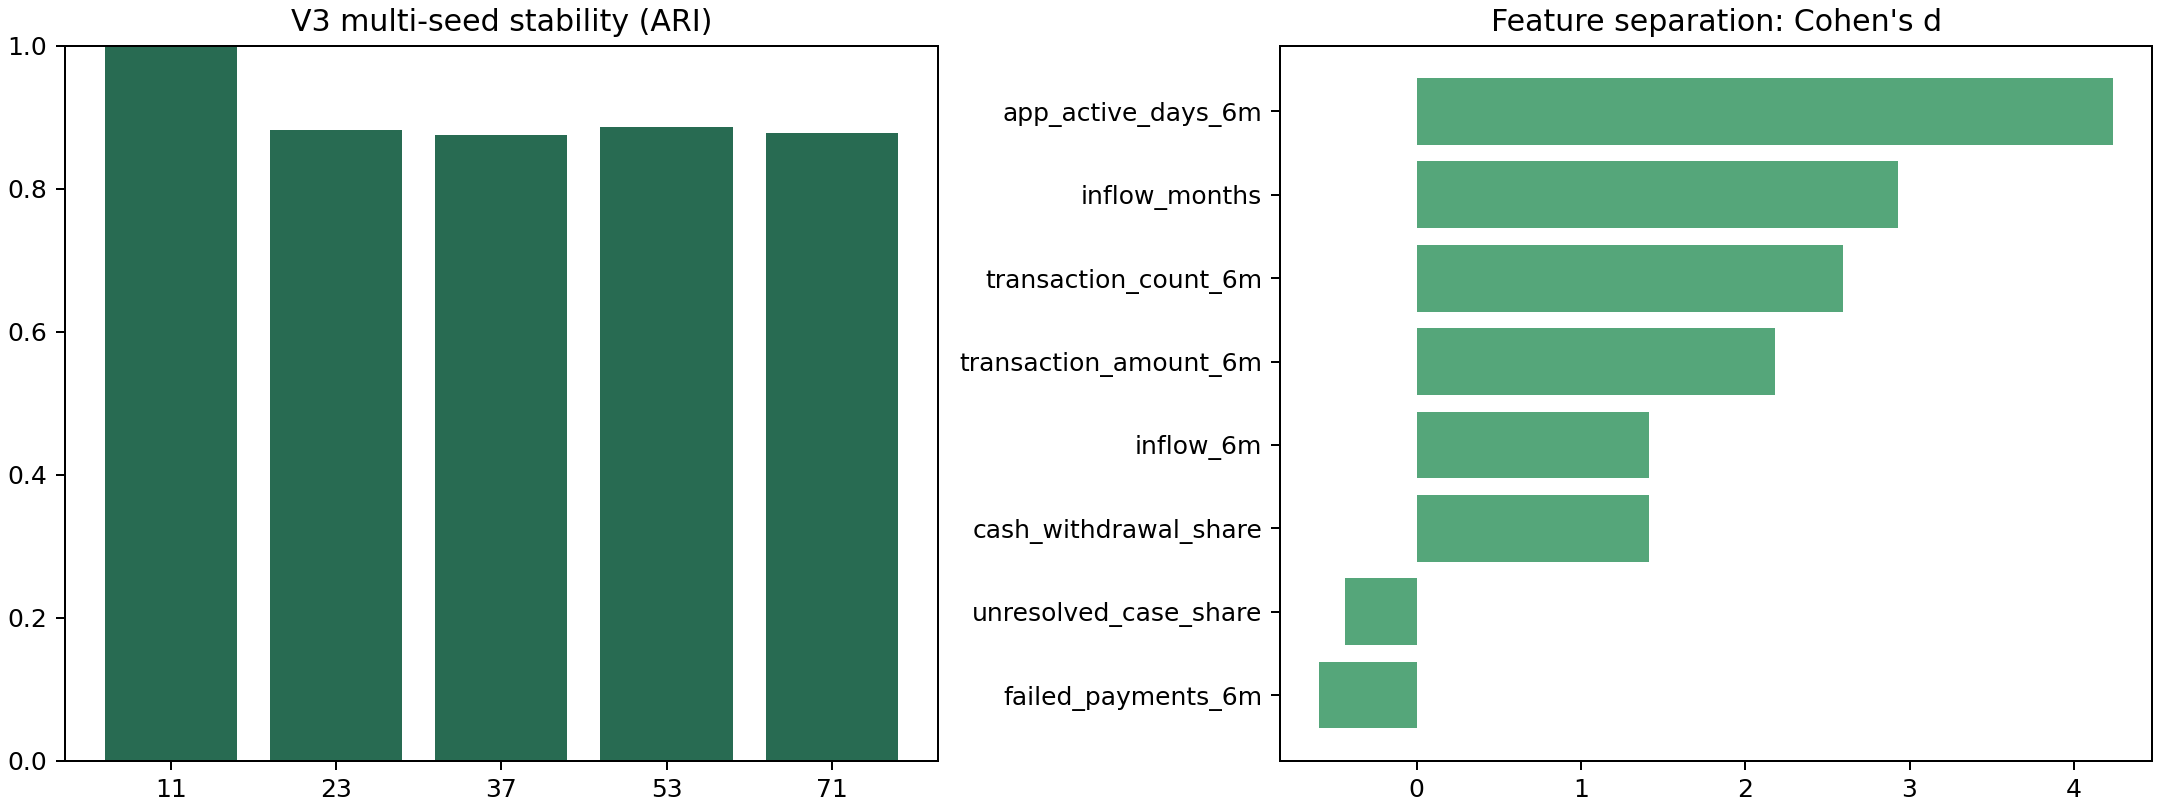
\includegraphics[width=0.95\textwidth]{figure/v3_stability_and_distinctiveness.png}
\caption{V3 stability across synthetic seeds and feature separation. Source: V3 synthetic-behaviour artifacts.}
\label{fig:stability}
\end{figure}

\begin{figure}[H]
\centering
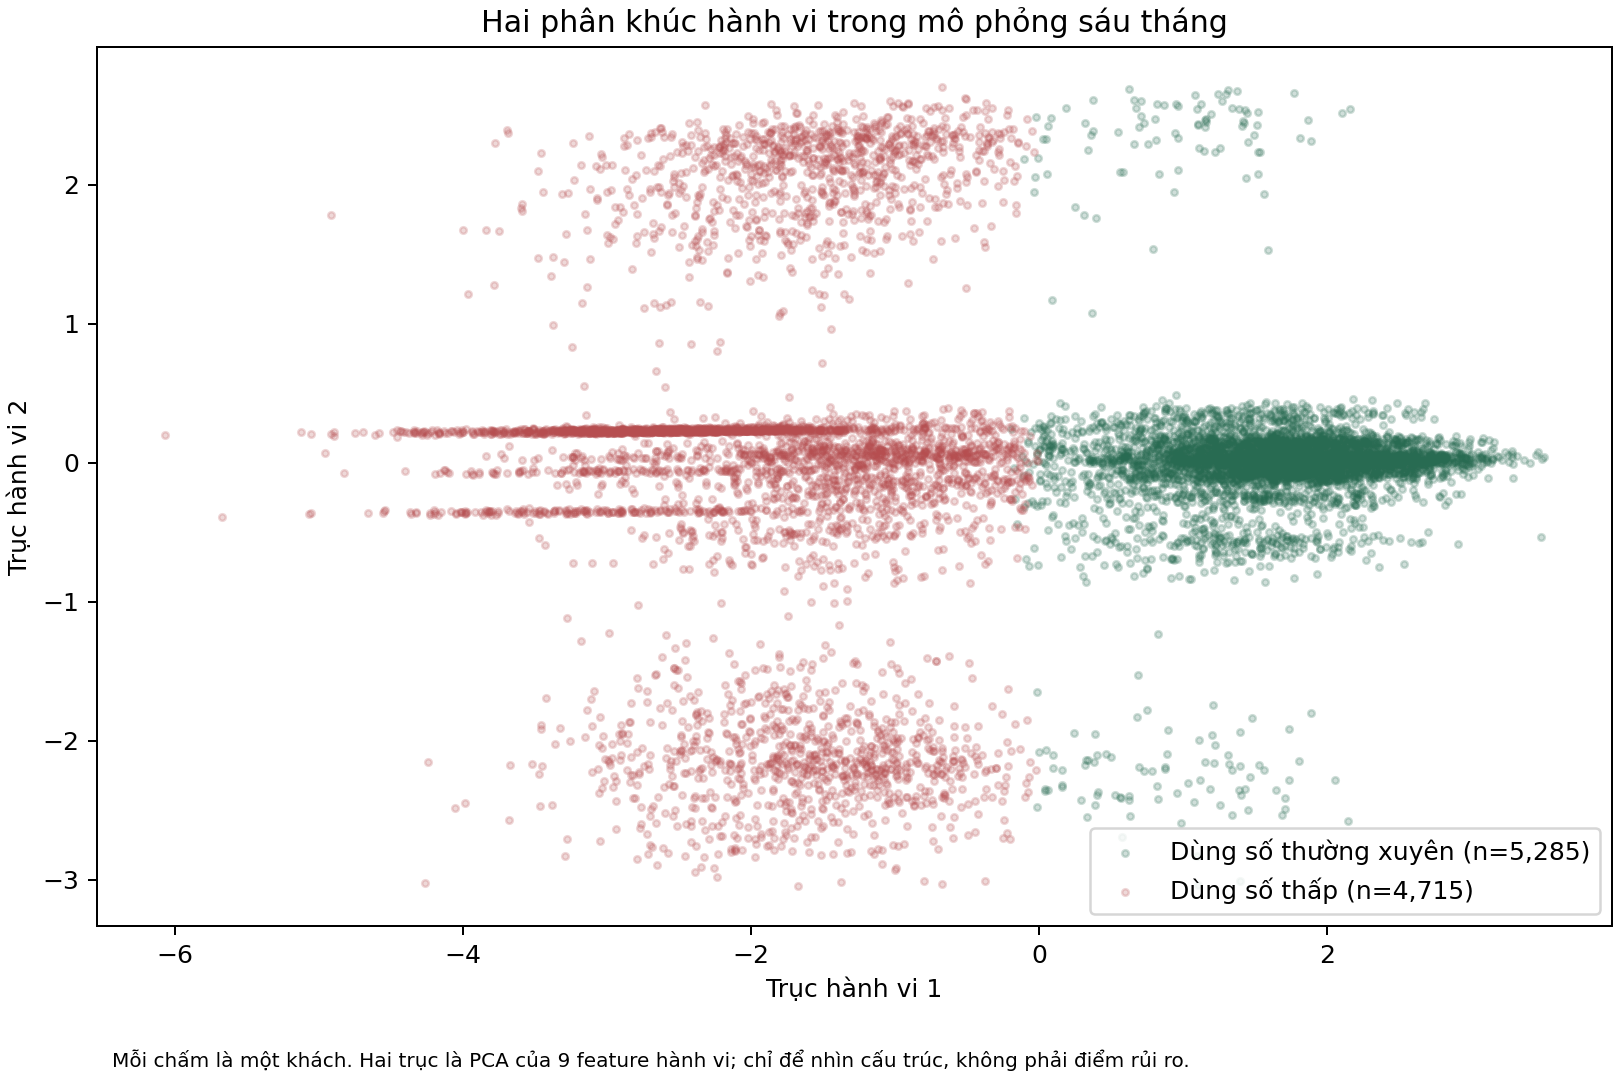
\includegraphics[width=0.80\textwidth]{figure/v3_cluster_map.png}
\caption{Two behavioural clusters in the V3 synthetic six-month window. Each point is one customer.}
\label{fig:clusters}
\end{figure}

\subsection{Persona 1: customers with an established digital routine}

This group contains 5,285 customers. Its static historical churn rate is 14.2\% (751 customers). Average age is 39.6 and average credit score is 653.2. In the simulation, customers open the app regularly, receive cash-flow events in more months, and complete more payment activity. Their common app tasks are transferring money, paying bills, checking balance and managing card controls. This is not proof of satisfaction. The operating risk is that friction in a routine task affects a large customer base before it appears as an explicit complaint.

The proposed experiment compares \emph{Digital Concierge}, contextual help during a routine task, with \emph{Value Review}, an opt-in explanation of current fees and benefits. The primary 90-day outcome is incremental retention; leading indicators are task completion, repeat support contact and opt-out. Customers with open service cases are suppressed from both arms.

\subsection{Persona 2: customers with a thin digital relationship}

This group contains 4,715 customers. Its static historical churn rate is 27.3\% (1,286 customers), 6.9 percentage points above the full cohort. Average age is 38.2 and average credit score is 647.5. In the simulation, customers open the app less often, use it mainly to inspect account status, receive incoming cash flow in fewer months, and show more failed-payment and unresolved-service signals. The simulation does not tell us why they may leave; it identifies a relationship that merits careful testing.

The proposed experiment compares \emph{Service Recovery}, a named owner and closure confirmation for a service issue, with \emph{Reactivation Coach}, a 14-day guided return to one useful action. An unresolved case always overrides marketing eligibility. The 90-day primary outcome is incremental active-month rate and retention; weekly guardrails are complaint, opt-out, failed-payment and case re-open rates.

\section{Churn prediction, solution architecture and recommendations}

The next project module will compare dummy, Logistic Regression, Random Forest and XGBoost under a leakage-safe static-label protocol. It will report ROC-AUC, PR-AUC, precision, recall, F1, calibration, threshold sensitivity and subgroup diagnostics. Scores will not be called next-quarter probabilities without real temporal labels.

The target product is a staff-facing dashboard and API with six layers: data quality; customer segments; churn intelligence; retention strategy; governance; and monitoring. The recommendation is to launch no customer contact until consent, suppression, sample-size, cost and outcome definitions are approved. The decision cube in Figure~\ref{fig:cube} illustrates how behavioural segment, service policy and simulated cash-flow scenario support capacity planning; cash-flow scenario is not a value tier.

\begin{figure}[H]
\centering
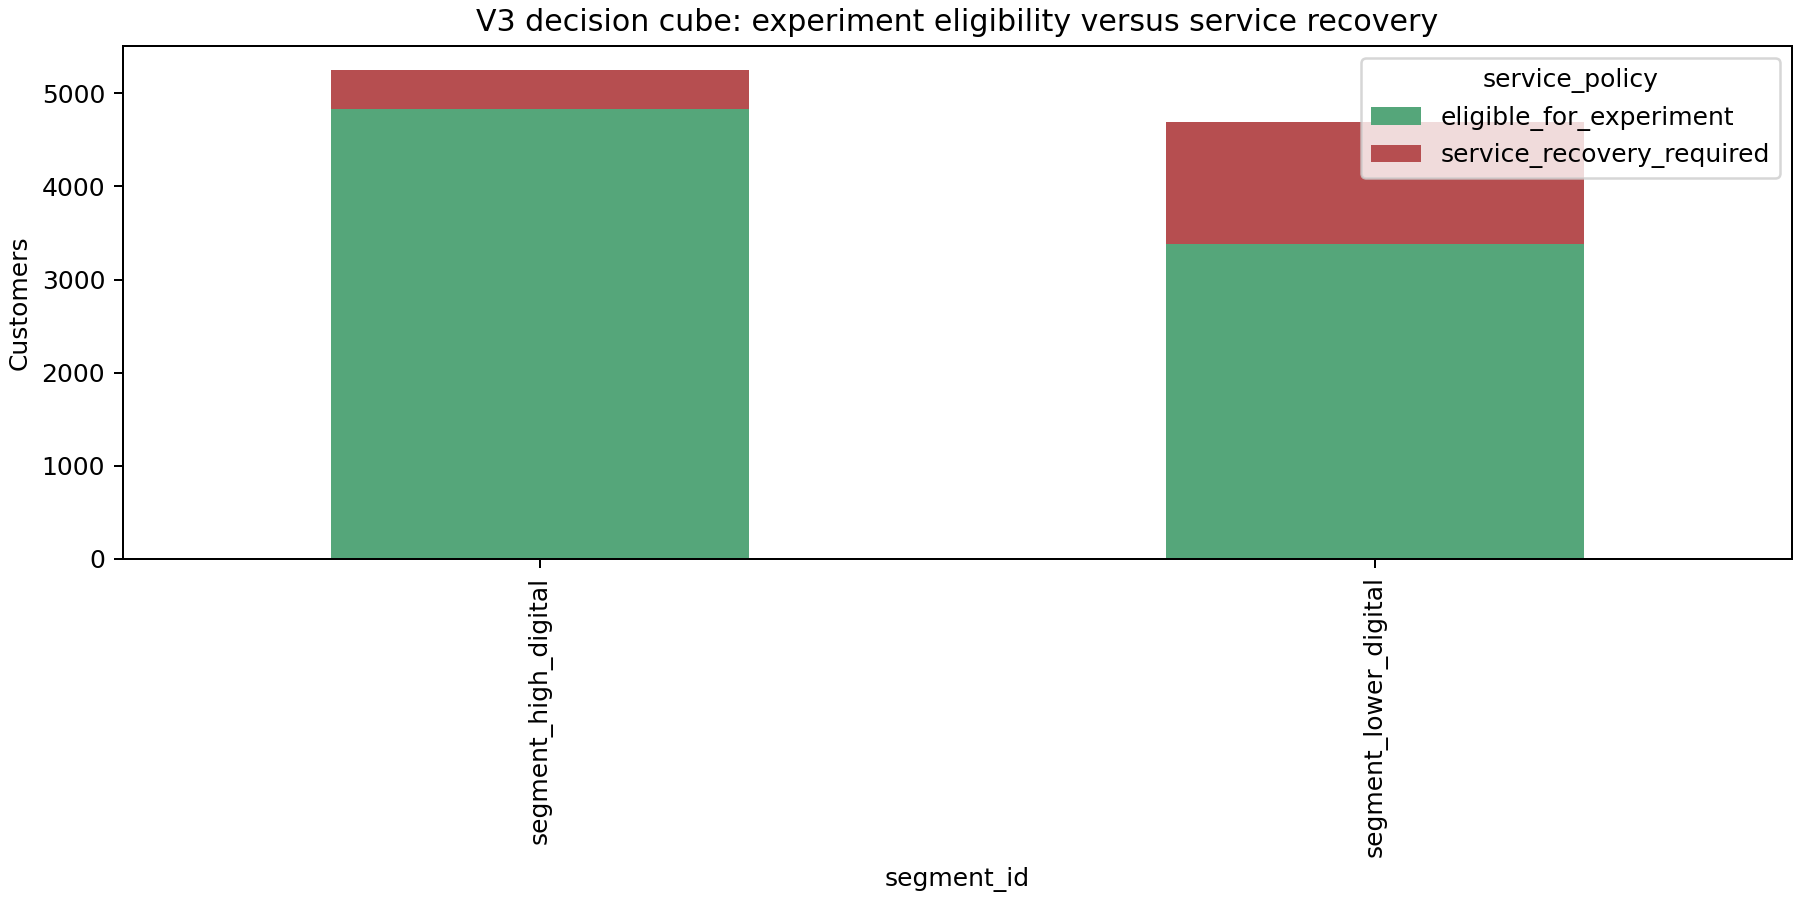
\includegraphics[width=0.82\textwidth]{figure/v3_decision_cube.png}
\caption{V3 decision cube for service routing and experiment eligibility.}
\label{fig:cube}
\end{figure}

